\documentclass{beamer}
\setbeamertemplate{caption}[numbered]
\usepackage{animate, lipsum, subfig}

\newcommand{\comment}[1]{}

\newcommand\blfootnote[1]{%
  \begingroup
  \renewcommand\thefootnote{}\footnote{#1}%
  \addtocounter{footnote}{-1}%
  \endgroup
}

% Load Packages
\usepackage[utf8]{inputenc}
\usepackage{xcolor}
\usepackage{tikz}
\usetikzlibrary{positioning,calc}
\usepackage{graphicx}
\usepackage{hyperref}
\usepackage{amsmath}
\usepackage{listings}
%\usepackage{fontawesome}

% Define Commands
\newcommand*{\ClipSep}{0.06cm} %To adjust footer logo
\newcommand{\E}{\mathrm{e}\,} %\def\I{e} % used to defined e for exp(x), see later what it should be
\newcommand{\ud}{\mathrm{d}}
\lstset{numbers=left, numberstyle=\tiny, stepnumber=1,firstnumber=1,breaklines=true,
    numbersep=5pt,language=Python,
    stringstyle=\ttfamily,
    basicstyle=\footnotesize, 
    showstringspaces=false
}

\usetheme{oxonian}

\title{LXe scintillation model}
\begin{document}

{\setbeamertemplate{footline}{} 
\frame{\titlepage}}

\begin{frame}{Objective}
The goal is is build a scintillation model for LXe: $Y_{a}(t,\hat{\theta})$.\\
$Y_{a}(t,\hat{\theta})$ is the probability to emit a photon at time $t$ to the direction $\hat{\theta}$. The subscript $a$ indicates the different type of interactions ($\gamma$, $N$, $\alpha$ and maybe different energies in the same interaction type).\\
\end{frame}


\begin{frame}{Signal Reconstruction}
%	\begin{center}
%	\animategraphics[loop,controls,width=0.6\linewidth]{10}{recon-}{0}{41}	
%	\end{center}
To study the temporal structure of the photon emission a processing algorithm uses a template of the average SPE signal to reconstruct the temporal PE pattern in each event for each PMT separately. The output of this process is the number of PEs created in the PMT in each digitization point.

\begin{figure}[h]
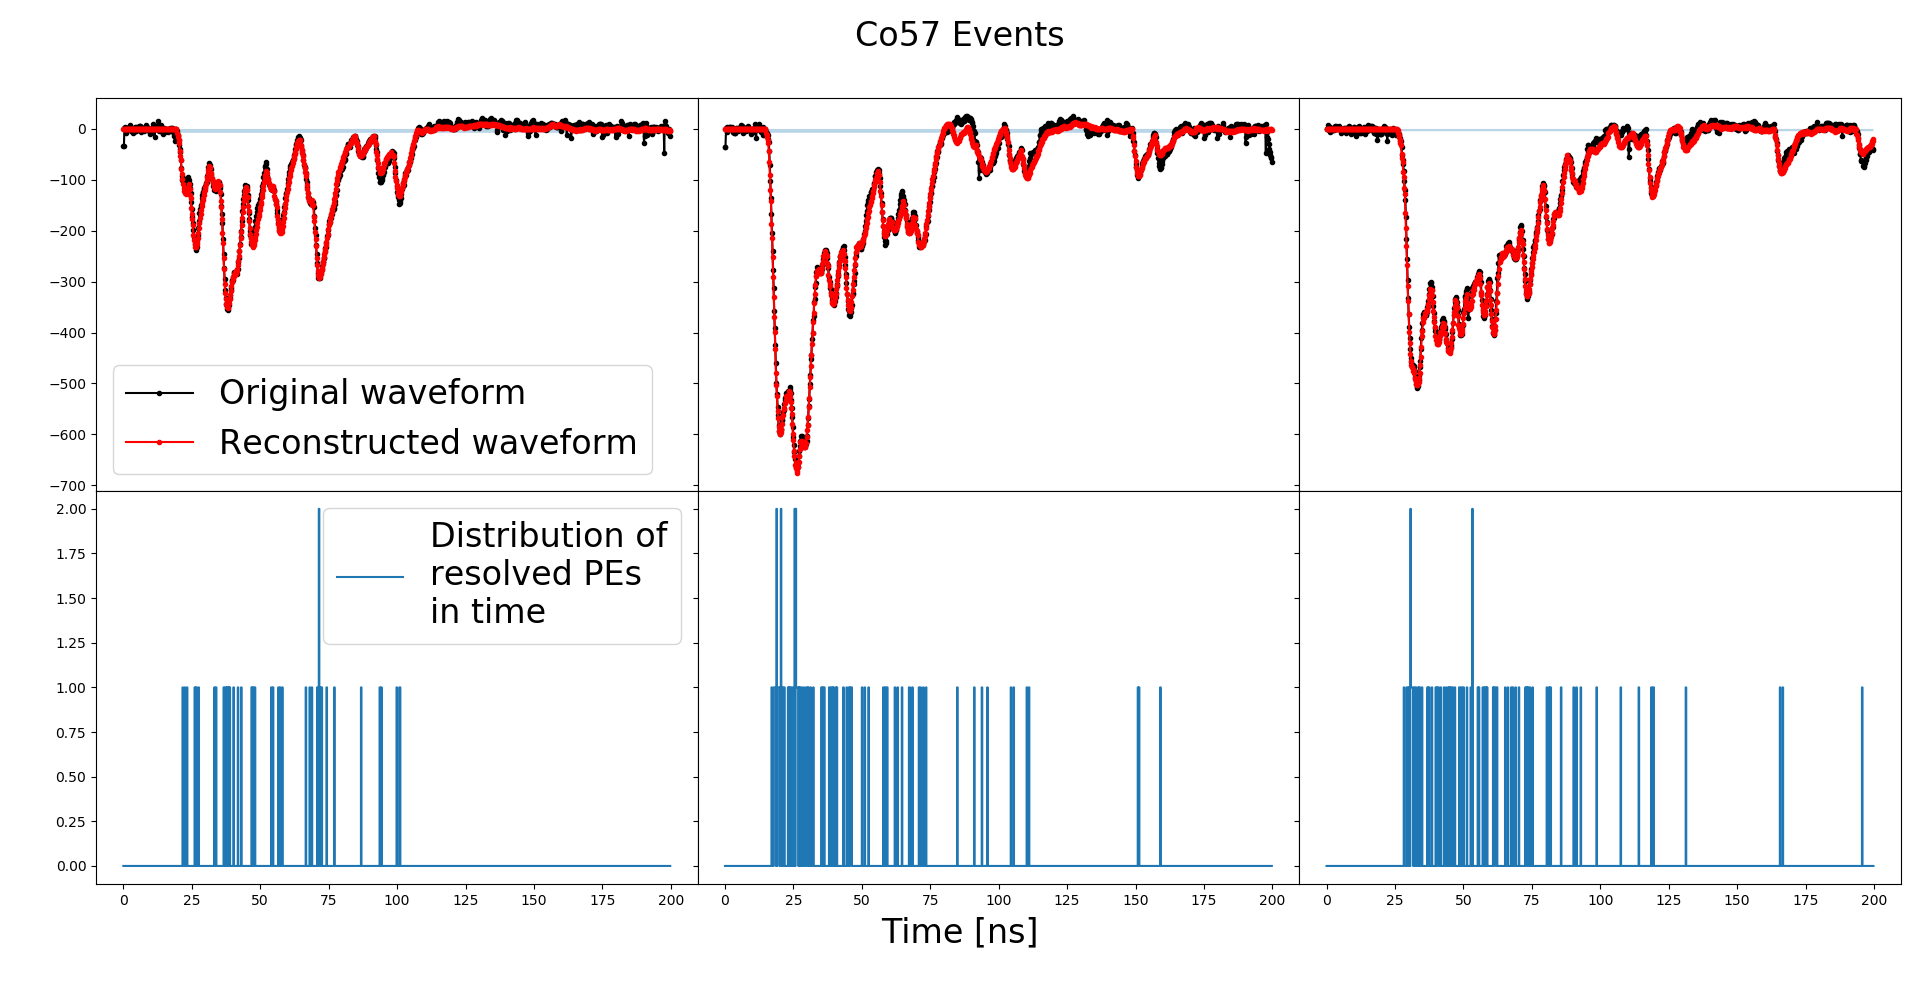
\includegraphics[width=1\textwidth]{recons.png}
\end{figure}

\end{frame}


\begin{frame}{Time Alignment Problem}
We do not know the "time zero" for each event due to two reasons:\\
\begin{itemize}
\item The trigger time is "random" so alignment by the trigger time would not help.
\item Alignment by the first resolved PE in the events: the resolved PEs time distribution is a random sample of the real emission times. We do not know the delay between the first resolved PE and the first photon that been emitted.
\end{itemize}
\begin{figure}[h]
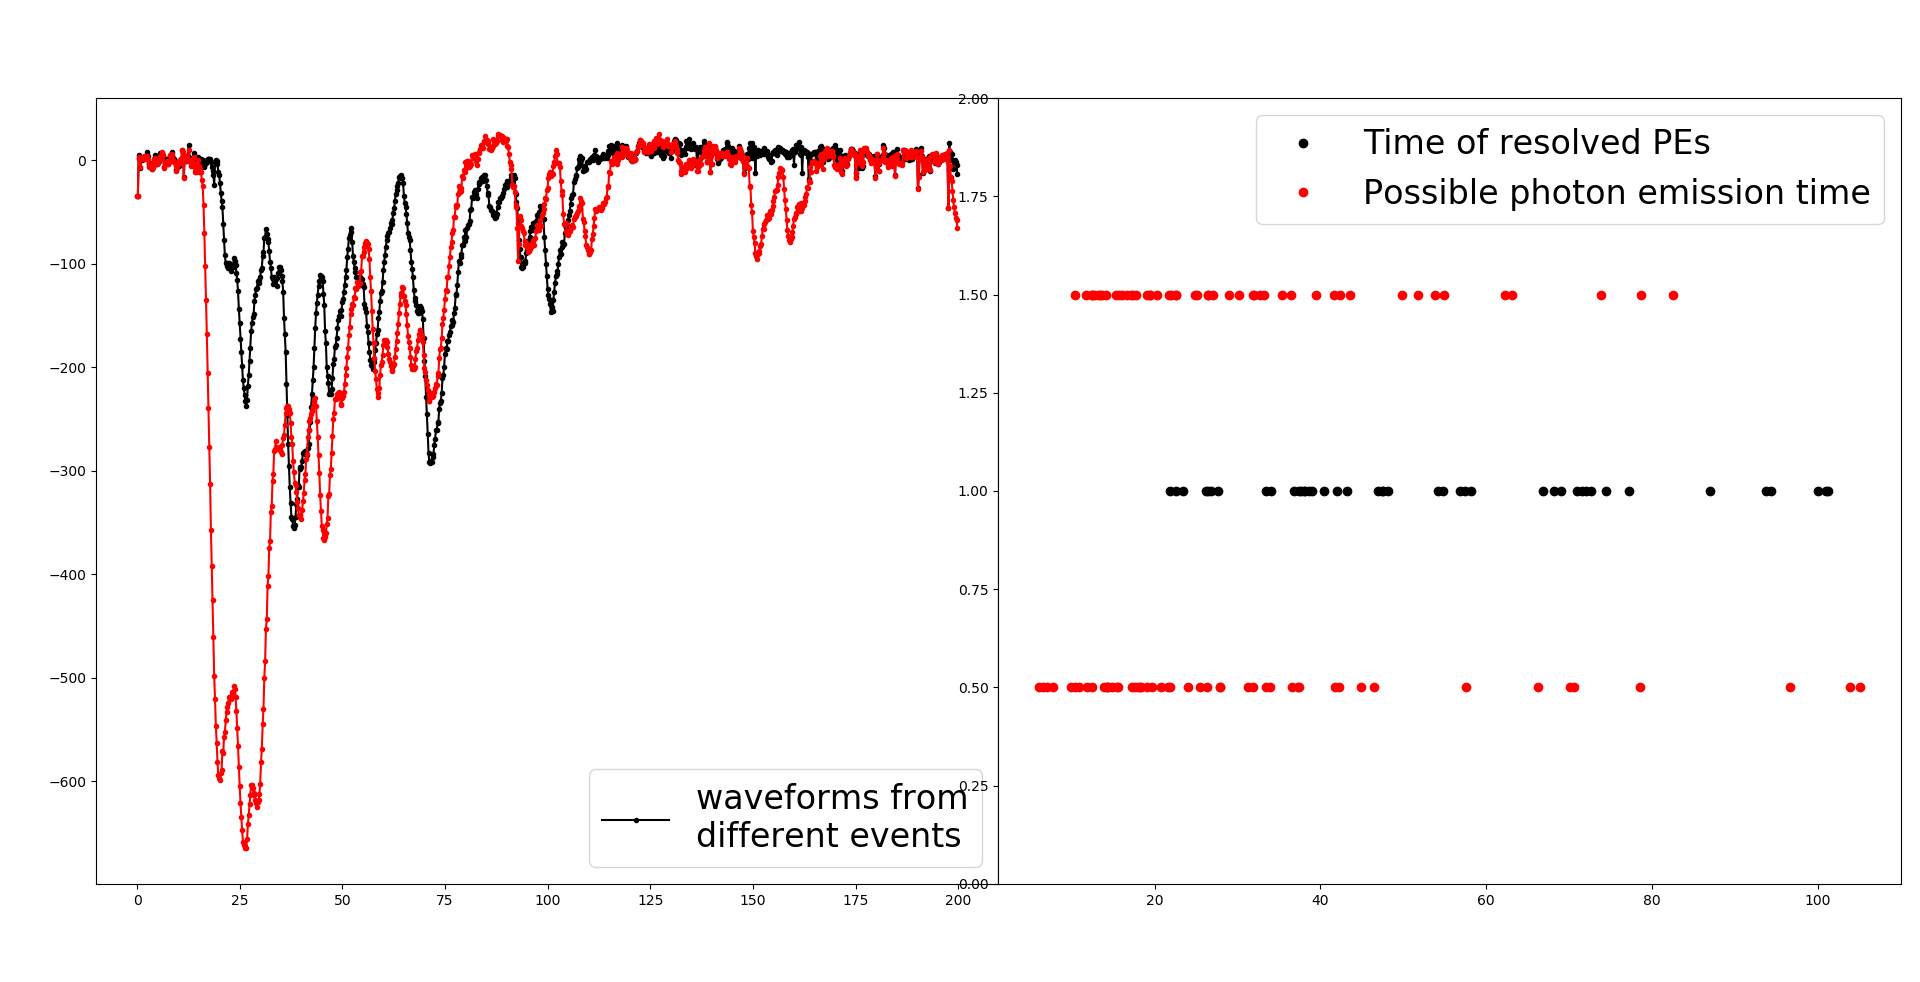
\includegraphics[width=0.6\textwidth]{alignment.png}
\end{figure}
\end{frame}

\begin{frame}{Time Alignment Problem}
Solution: Align by the first resolved photon and adjust the model from probabilities of photon emission times to probabilities of time difference between photons.  
\begin{figure}[h]
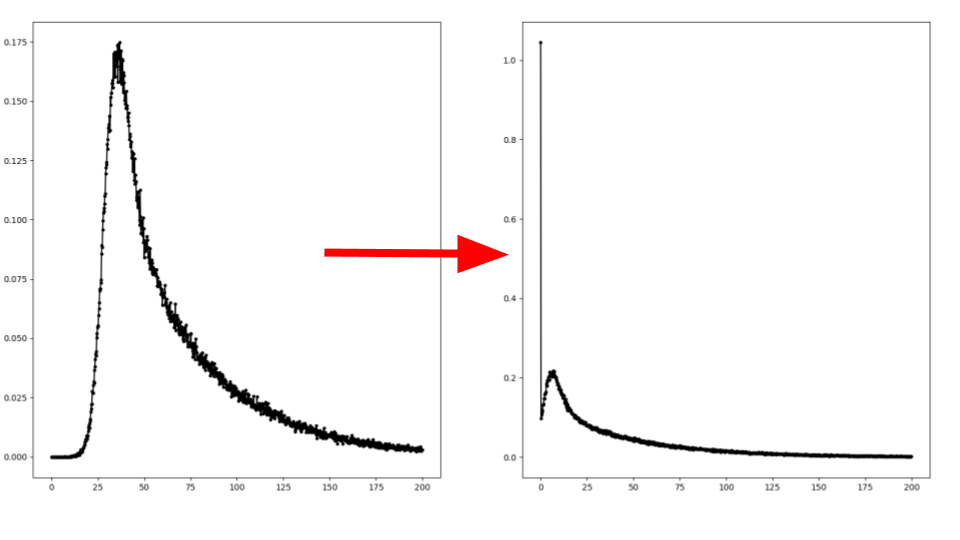
\includegraphics[width=0.6\textwidth]{sim1.png}
\label{sim_temp}
\caption{Mean temporal distribution of 10K simulated events (two exponential decay model). Left is no aligned at all so the fast component is smeared by the jitter of the trigger. Right is all the events aligned by the first PE in the events. The pole at 0 represents the fact that in each event the number of PEs resolved at time 0 is greater then 0 (by definition). More about the simulation in next slides.}
\label{sim_temp} 
\end{figure}
\end{frame}

\begin{frame}{Spoiler}
This is how the temporal distribution from $^{57}$Co events looks like on two PMTs:
\begin{figure}[h]
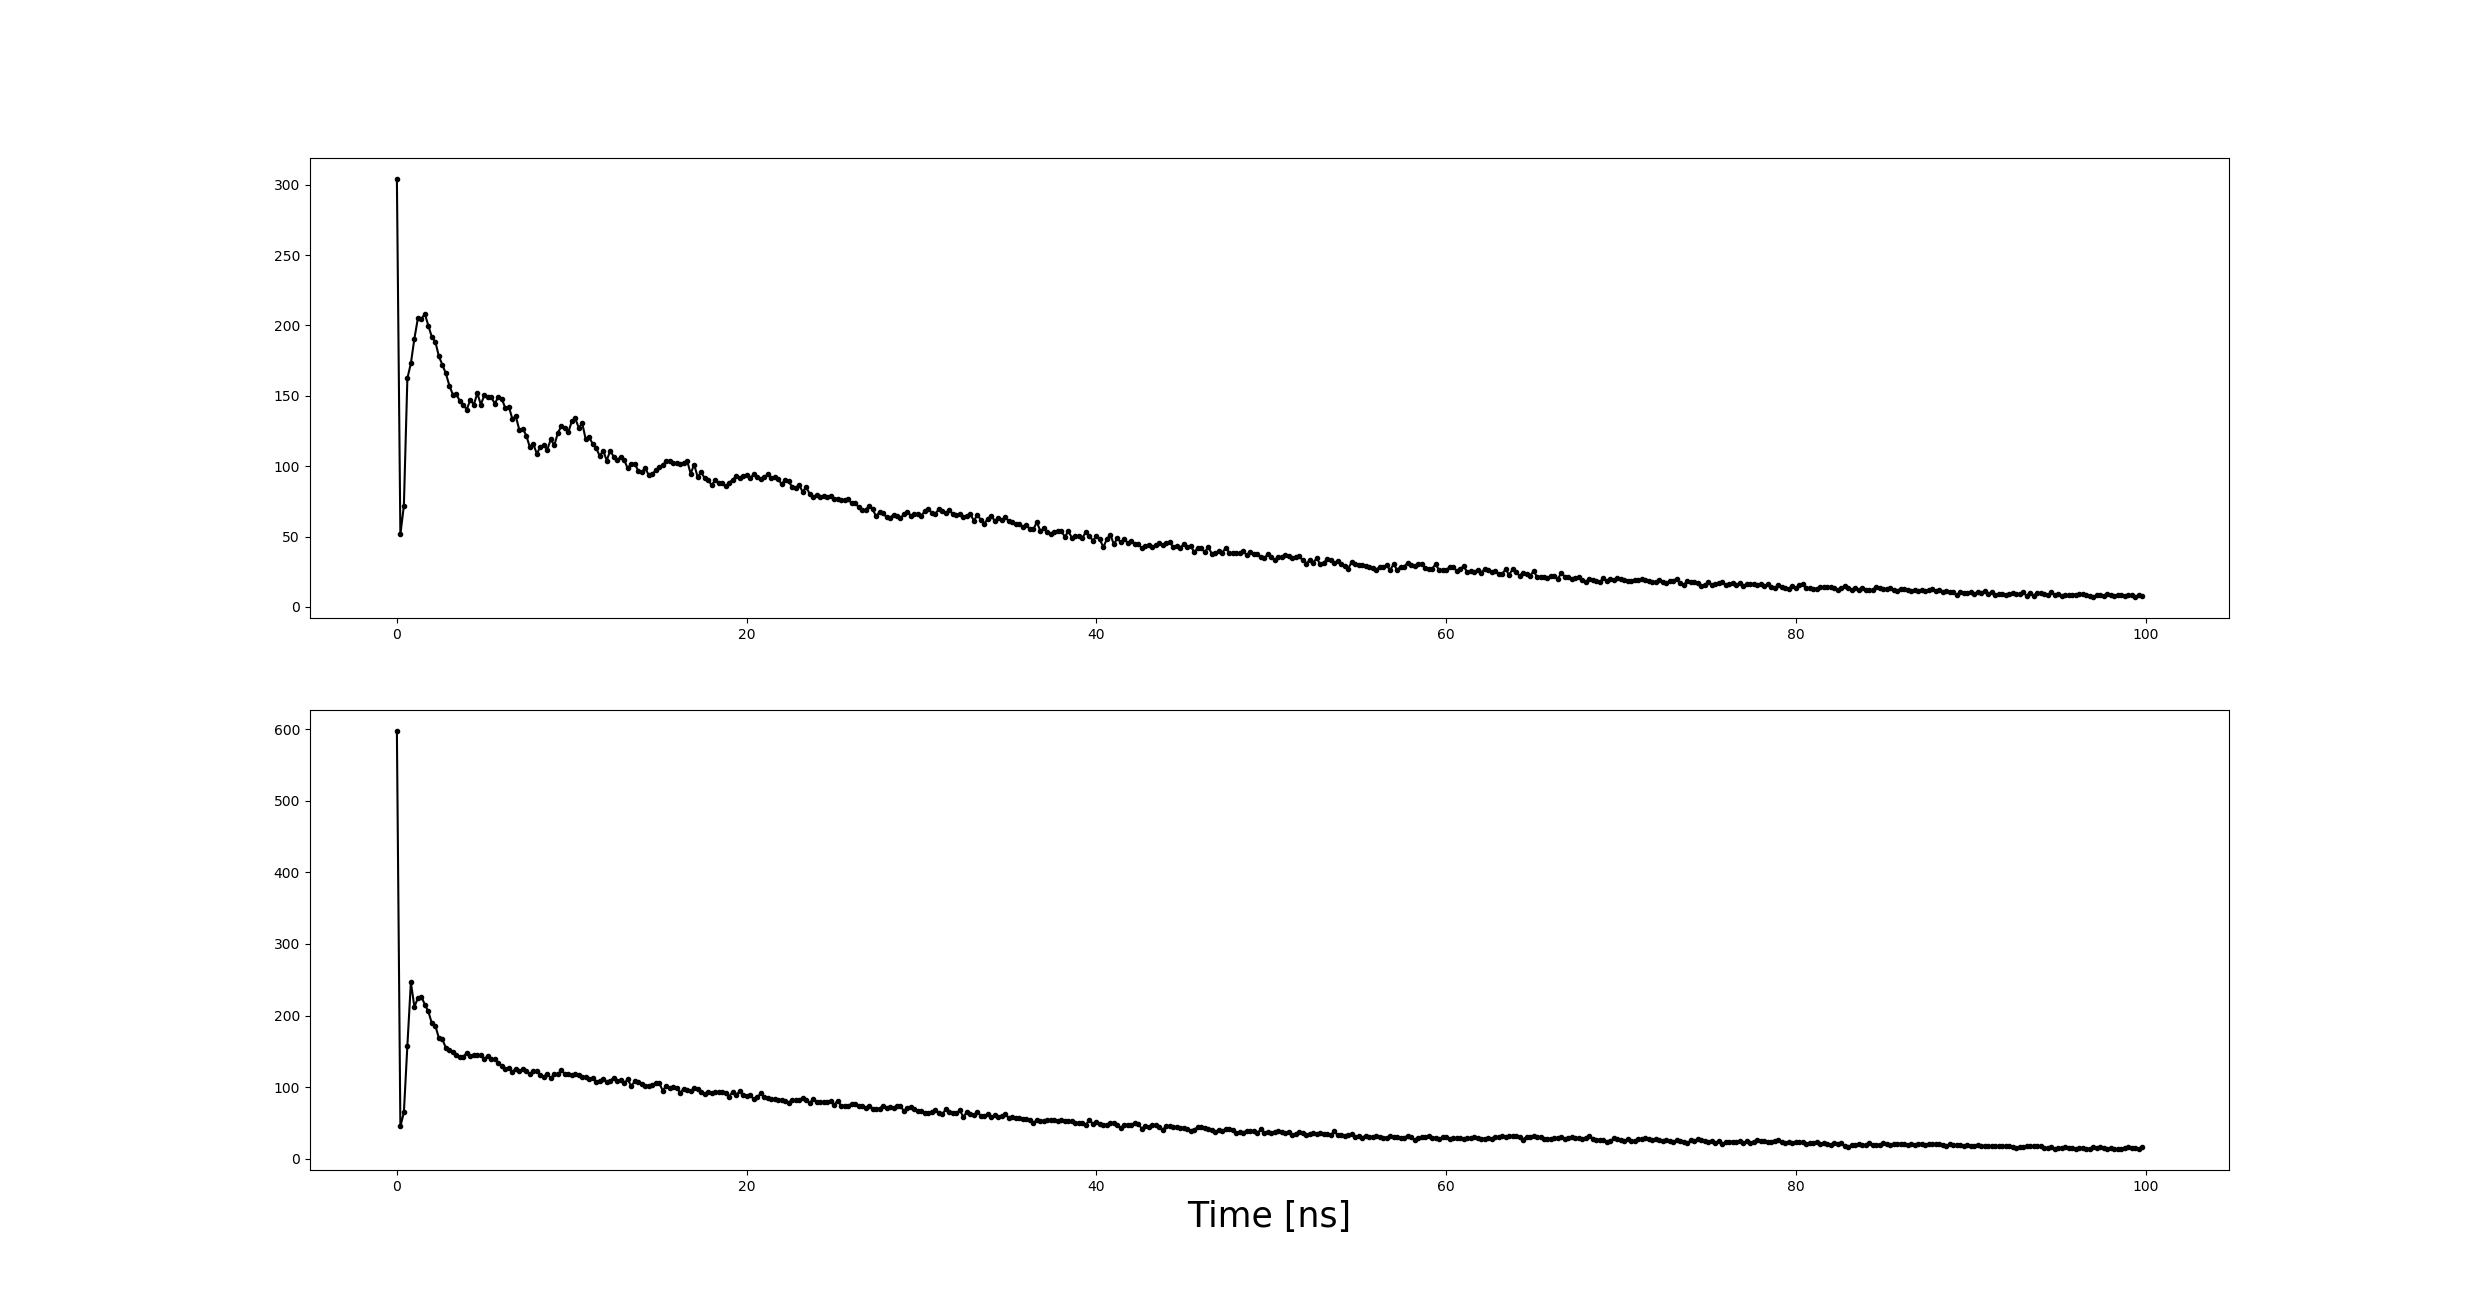
\includegraphics[width=1\textwidth]{temporal1.png}
\end{figure}
\end{frame}

\begin{frame}{PE Histogram}
The observable that we want to build a model for is a 2D histogram (for each PMT and each interaction type) $H_{ni}$ which holds the number of events in which $n$ PEs where resolved at time $t_i$ after the first resolved PE in that events.

\blfootnote{$\sum_nnH_{ni}$ is the right panel in figure~\ref{sim_temp}.}

\end{frame}

\begin{frame}{Scintillation Model}
The number of photons emitted at the time window $[t_i, t_i+dt_i]$ is distributed Poisson,
\begin{equation}
n_i^{ph}\sim\text{Poisson}(Y_a(t_i)N_adt_i)
\end{equation} 
where $N_a$ is the average number of photons generated by event type $a$ and $Y_a(t_i)$ is the probability to emit a photon at time $t_i$.
The number of PEs created in the time window is
\begin{equation}
n_i^{pe}\sim\text{Binom}(Q,\text{Poisson}(Y_a(t_i)N_adt_i)),
\end{equation}
where $Q$ is the photon detection efficiency (quantum efficiency, collection efficiency, double PE probability..., all the mechanisms that takes $m$ photons and convert them to $n<m$ PEs).
\end{frame}

\begin{frame}{Scintillation Model}
Each PMT has its temporal uncertainty combined with the code's temporal uncertainty. $\tilde{n}_i$ - the number of PEs that resolved at time window $t_i$ is a sum of a random variables $m_{ij}$ that represents the number of PEs that were created at time $t_j$ but were resolved at time $t_i$:
\begin{equation}
\begin{split}
m_{ij}&\sim n^{pe}_jdt_i\text{Norm}(t_i|T_0+t_j, \sigma_t),\\
\tilde{n}_i&\sim\sum_{j\in\text{all digi points}}m_{ij},
\end{split}
\end{equation}
where $T_0$ is the time when the events started in the digitization window and $\sigma_t$ is the temporal uncertainty of each PMT.
\blfootnote{$m_{ij}$ is kind of ill-defined with the normal distribution which gives non-integer values, but its need to be though in the sense that as the temporal uncertainty is larger there is a higher probability to resolve a bigger fraction of $n_j^{pe}$ at a different time.}
\end{frame}

\begin{frame}{Scintillation Model}
Since $\tilde{n}_i$ is a sum of independent random variables its distribution can be approximated by a different distribution with mean and variance which are the sum of the means and variances of $m_{ij}$,
\begin{equation}
\begin{split}
\langle\tilde{n}_i\rangle&=\sum_j\langle m_{ij}\rangle\\
\text{Var}(\tilde{n}_i)&=\sum_j\text{Var}(m_{ij})
\end{split}
\end{equation}
Plug in the given $n_j^{pe}$ and compute the mean and the variance of $m_{ij}$ you get
\begin{equation}
\langle m_{ij}\rangle=\text{Var}(m_{ij})=QN_adt_idt_jY_a(t_j)\text{Norm}(t_i|T_0+t_j, \sigma_t).
\end{equation}
\end{frame}

\begin{frame}{Scintillation Model}
The average and the variance of $\tilde{n}$ are equal so we assume its distributed Poisson
\begin{equation}
\begin{split}
\tilde{n}_i\sim&\text{Poisson}\left(QN_adt_idt_j\sum_jY_a(t_j)\text{Norm}(t_i|T_0+t_j, \sigma_t)\right)=\\
&\text{Poisson}\left(QN_adt_i\int Y_a(t_j)\text{Norm}(t_i|T_0+t_j, \sigma_t)dt_j\right).
\end{split}
\end{equation}
\end{frame}

\begin{frame}{Scintillation Model}
If we will take $Y_a(t_i)$ as a sum exponential decaying components
\begin{equation}
Y_a(t_j)=\sum_c\frac{F_c}{\tau_c}e^{-t_j/\tau_c} \quad (\sum_cF_c=1)
\end{equation}
we will get 
\begin{equation}
\begin{split}
&\int Y_a(t_j)\text{Norm}(t_i|T_0+t_j, \sigma_t)dt=\\
&\sum_c\frac{F_cK_c}{\tau_c}e^{-t_i\tau_c}\left[1-\text{erf}\left(\frac{\sigma_t}{\sqrt{2}\tau_c}-\frac{t_i-T_0}{\sqrt{2}\sigma_t}\right)\right]
\end{split}
\end{equation}
where $K_c$ is a normalization factor
\begin{equation}
K=\left[1-\text{erf}\left(\frac{\sigma_t}{\sqrt{2}\tau}+\frac{T_0}{\sqrt{2}\sigma_t}\right)+e^{-\sigma_t^2/2\tau^2-T_0/\tau}\left(1+\text{erf}\left(\frac{T}{\sqrt{2}\sigma_t}\right)\right)\right]^{-1}
\end{equation}
\end{frame}

\begin{frame}{Scintillation Model with $\delta(t)$}
If we want to add a super fast component in the beginning of the model it is represented by
\begin{equation}
Y_a(t)=(1-R_\delta)\sum_c\frac{F_c}{\tau_c}e^{-t/\tau_c}+R_\delta\delta(t),
\end{equation}
So we need to add to equation 8 from the previous slide:
\begin{equation}
\frac{R_\delta}{\sqrt{2\pi}\sigma_t}e^{-(t-T_0)^2/(2\sigma_t^2)}
\end{equation}
\end{frame}

\begin{frame}{Scintillation Model - Alignment}
Recall that we build a model for $H_{ni}$ which holds the number of events in which $n$ PEs were resolved at time $t_i$ after the first resolved PE.
Without the alignment problem, naively, 
\begin{equation}
\tilde{H}_{ni}=N_{\text{events}}\text{Poisson}\left(n\bigg|\lambda=QN_adt\int Y_a(t_j)\text{Norm}(t_i|T_0+t_j, \sigma_t)dt\right)
\end{equation}
\blfootnote{$\tilde{H}_{ni}$ is $H_{ni}$ before the alignment. The naively comment states that we also need to account the uncertainty in the number of PEs resolved, i.e the probability to resolve $n$ PEs where $m$ where actually extracted. This is related to the width of the SPE area distribution  and will be treated later.}
\end{frame}

\begin{frame}{Alignment for $i>0$}
The model $\tilde{H}_{ni}$ tells us what is the probability that $n$ PEs will be resolved at time $t_i$. So 
\begin{equation}
\begin{split}
H_{ni}=\sum_j&[\text{Non of the PMTs resolved a PE untill time }t_j]\times\\
&[\text{Some PMT resolved a PE (or more) at time }t_j]\times\\
&\tilde{H}_{ni+j}
\end{split}
\end{equation}
\end{frame}

\begin{frame}{Alignment for $i>0$}
\begin{equation}
\begin{split}
&[\text{Non of the PMTs resolved a PE untill time }t_j]=\\
&\prod_{\text{all PMTs}}\prod_{k<j}\tilde{H}_{0k}^{\text{pmt}}
\end{split}
\end{equation}
\begin{equation}
\begin{split}
&[\text{Some PMT resolved a PE (or more) at time }t_j]=\\
&\sum_{\text{pmt}}[1-\tilde{H}_{0j}^{\text{pmt}}]
\end{split}
\end{equation}

\blfootnote{The superscript pmt indicates the product on all PMTs (each pmt has a different model).}
\end{frame}

\begin{frame}{Alignment for $i>0$}
\begin{equation}
H_{ni}=\sum_j\prod_{\text{all PMTs}}\prod_{k<j}\tilde{H}_{0k}^{\text{pmt}}\sum_{\text{pmt}}[1-\tilde{H}_{0j}^{\text{pmt}}]\tilde{H}_{ni+j}
\end{equation}
\end{frame}

\begin{frame}{Alignment for $i=0, n>0$}
In this case we dont need the middle term in the previous slide (which represents the probability that the first PE was resolved at time $t_j$), So for $n>0$
\begin{equation}
H_{n0}=\sum_j\prod_{\text{all PMTs}}\prod_{k<j}\tilde{H}_{0k}^{\text{pmt}}\tilde{H}_{nj}
\end{equation}
\end{frame}

\begin{frame}{Alignment for $i=0, n=0$}
Here we do need the middle term but we dont want to sum on the pmt of interest. So
\begin{equation}
H_{00}^{\text{pmt}_0}=\sum_j\prod_{\text{all PMTs}}\prod_{k<j}\tilde{H}_{0k}^{\text{pmt}}\sum_{\text{pmt}\neq\text{pmt}_0}[1-\tilde{H}_{0j}^{\text{pmt}}]\tilde{H}_{0j}^{\text{pmt}_0}
\end{equation}
\end{frame}

\begin{frame}{First Look at Data}
I ran the reconstruction algorithm on the $^{57}$Co dataset with PMTs 7 and 8. In each event the two signals were aligned by the delay that was measured by the pulser data. After reconstruction the temporal pattern of the resolved PEs was aligned ones more relative to the first PE resolved (in PMT 7 or 8). The events in which the $\chi^2$ of the reconstructed signal relative to the signal was too big were cut out. Also events with large baseline width were cut out. A range in the energy spectrum (number of resolved PEs) of each PMT was chosen and from these events a 2D histogram was made for each PMT ($D_{ni}^{\text{pmt}}$) which holds the number of events in which $n$ PEs was resolved at time $t_i$ after the first resolved PE.
\blfootnote{Maybe it is better to choose events from the combined distribution, i.e if an events is cut in one PMT it should be cutted out of all the PMTs.} 
\end{frame}

\begin{frame}{First Look at Fit - Double Exp Model}
\begin{figure}[h]
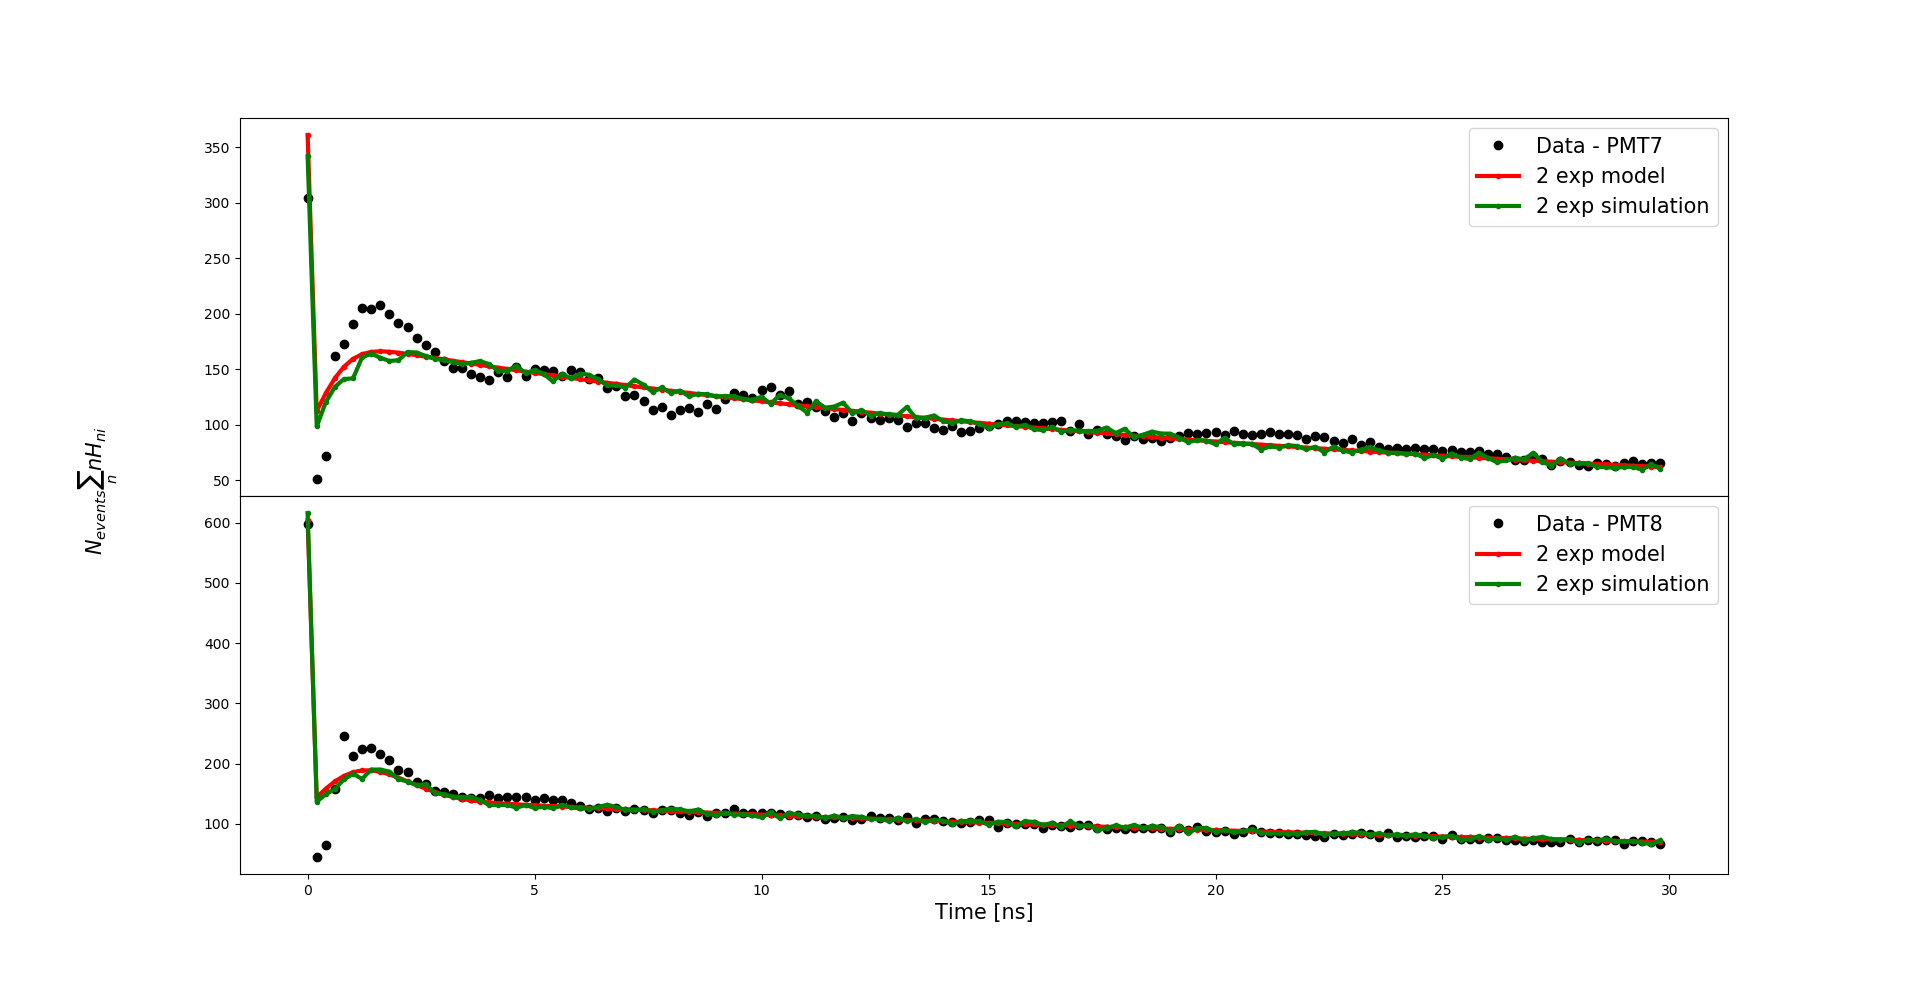
\includegraphics[width=1\textwidth]{fit1.png}
\end{figure}

\begin{center}
\begin{tabular}{|c||c|c|c|c|c|c|} 
\hline
PMT & $NQ$ & $T_0$ [ns]& $\sigma_t$ [ns] & $F$ & $\tau_f$ [ns] & $\tau_s$ [ns]\\ 
\hline\hline
7 & 34.5 & 39.9 & 0.4 & 0.2 & 15.6 & 44 \\
\hline
8 & 34.8 & 40.5 & 1 & 0.05 & 0.15 & 39.6 \\
\hline
\end{tabular}
\end{center} 
\end{frame}

\begin{frame}{First Look at Fit - Double Exp Model}
We see that the model doesn't fit perfectly the data but at list the simulation and the model give the same temporal structure which indicates that the analytical model represents the physics we try to model. Its a good point to talk about the simulation.
\end{frame}

\begin{frame}{Simulation 1}
the simulation creates the temporal structure of 10K events on two PMTs. Align the events by the first PE and finally creates a simulated 2D Histogram for each PMT ($S_{ni}$) which holds the number of simulated events in which $n$ PEs were created at time $t_i$ after the first PE. 
For each simulated event:
\begin{itemize}
\item A trigger time ($t_{trig}$) is sampled out of a normal distribution with mean 0 and variance $\sigma_{trig}^2$. This trigger is common for all PMTs.
\item For each PMT ($a$) a total number of PEs in event ($n^a$) is sampled out of Poisson distribution with mean $NQ^a$.
\item For each PMT the $n^a$ PEs are grouped in two groups $n_f, n_s$ (three groups with $n_\delta$ if we want to simulate a $\delta(t)$ pulse). The occupancy of each group sampled from distribution with probabilities $F, 1-F$ (and $R_\delta^a$ for the $\delta$ model). 
\end{itemize}
\end{frame}

\begin{frame}{Simulation 1}
\begin{itemize}
\item For each PMT, $nf$ times ($t_f$) are sampled from an exponential distribution with decay constant $\tau_f$, and $ns$ times ($t_s$) are sampled from an exponential distribution with decay constant $\tau_s$.
\item For each PMT smear the two exponential component by sampling for each sampled time $t_{f/s}^i\rightarrow \text{Normal}(\text{mean}=t_{trig}+T_0^a+t_{f/s}^i, \text{Var}=(\sigma_t^a)^2)$
\item Find the minimal time over all PMTs (global for event) and roll all times back relative to this time.
\end{itemize}
\end{frame}

\begin{frame}{First Look at Fit - $\delta(t)+$ Double Exp Model}
\begin{figure}[h]
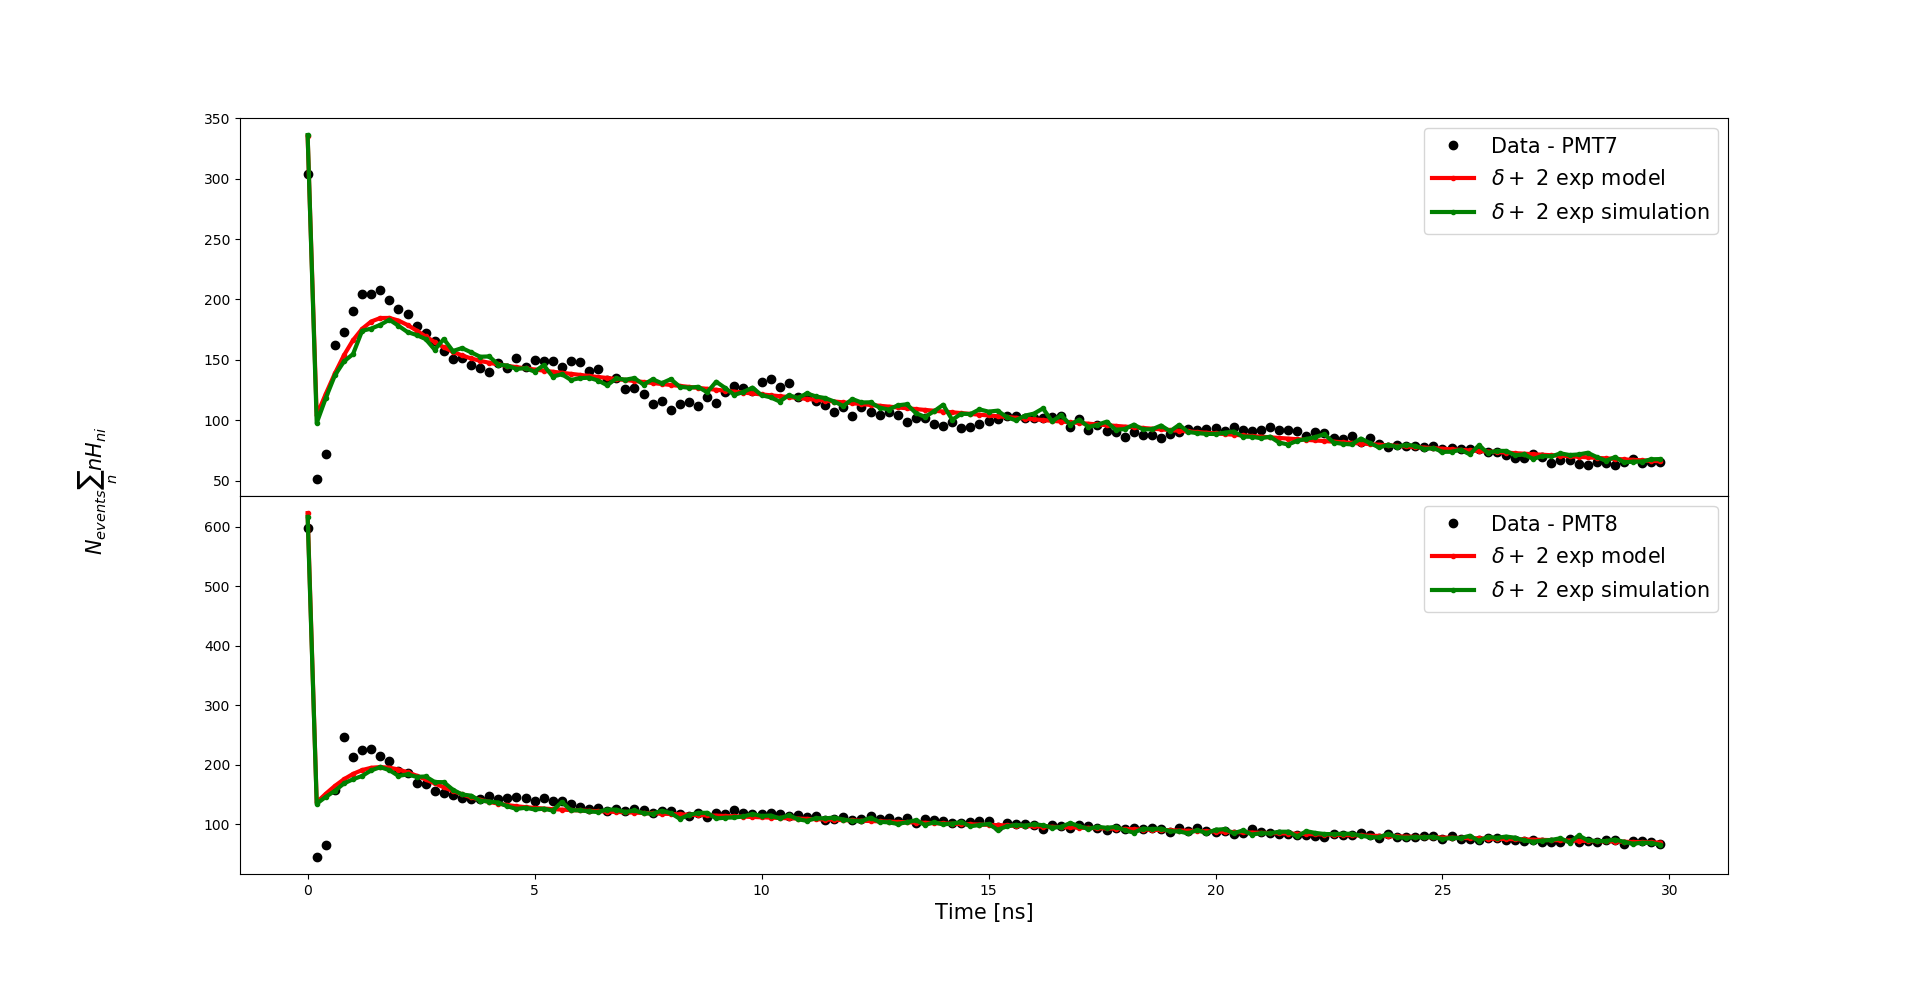
\includegraphics[width=1\textwidth]{fit2.png}
\end{figure}

\begin{center}
\begin{tabular}{|c||c|c|c|c|c|c|c|} 
\hline
PMT & $NQ$ & $T_0$ [ns]& $\sigma_t$ [ns] & $R$ & $F$ & $\tau_f$ [ns] & $\tau_s$ [ns]\\ 
\hline\hline
7 & 33.6 & 40.9 & 0.7 & 0.04 & 0.06 & 19.7 & 34.1 \\
\hline
8 & 35.1 & 40.8 & 1.14 & 0.01 & 0.04 & 0.17 & 41.2\\
\hline
\end{tabular}
\end{center}

\end{frame}

\begin{frame}{$\delta(t)+$ Double Exp Model - $F, \tau_f, \tau_s$ Global}
It make sense that $F, \tau_f$ and $\tau_s$ are not directional, i.e all PMTs should see the same values. When I tried to fit the data with this values globally for both PMTs I got weird results ($\tau_s\sim200$ [ns], both $\sigma_t>1$ [ns]). To mitigate this I fitted the data of the hit times of the PEs ($D^{\text{pmt}}_{ni}$) simultaneously with the delays distribution between SPE hits acquired from the calibration data and with correction for dark current. The model I used for the delay distribution is
\begin{equation}
\text{Delay}_{ij}=a_{delay}\text{Normal}\left(\text{mean}=T_{0,i}-T_{0,j}, \text{Var}=\left(\sigma_{t,i}^2+\sigma_{t,j}^2\right)\right).
\end{equation}

\end{frame}

\begin{frame}{Dark Current}
The reconstruction algorithm some time reconstruct a PE where it should not be. The rate of this falls reconstructions is the dark current ($f_{dc}$). The probability to have $n>0$ dark PEs at a digi point is $f_{dc}^n$ and the probability to 0 dark PEs in a digi point is $1-\frac{f_{dc}}{1-f_{dc}}$. This parameter can be calibrated from the pulser data by applying the reconstruction algorithm out of the time window where the SPE is expected.
\begin{figure}[h]
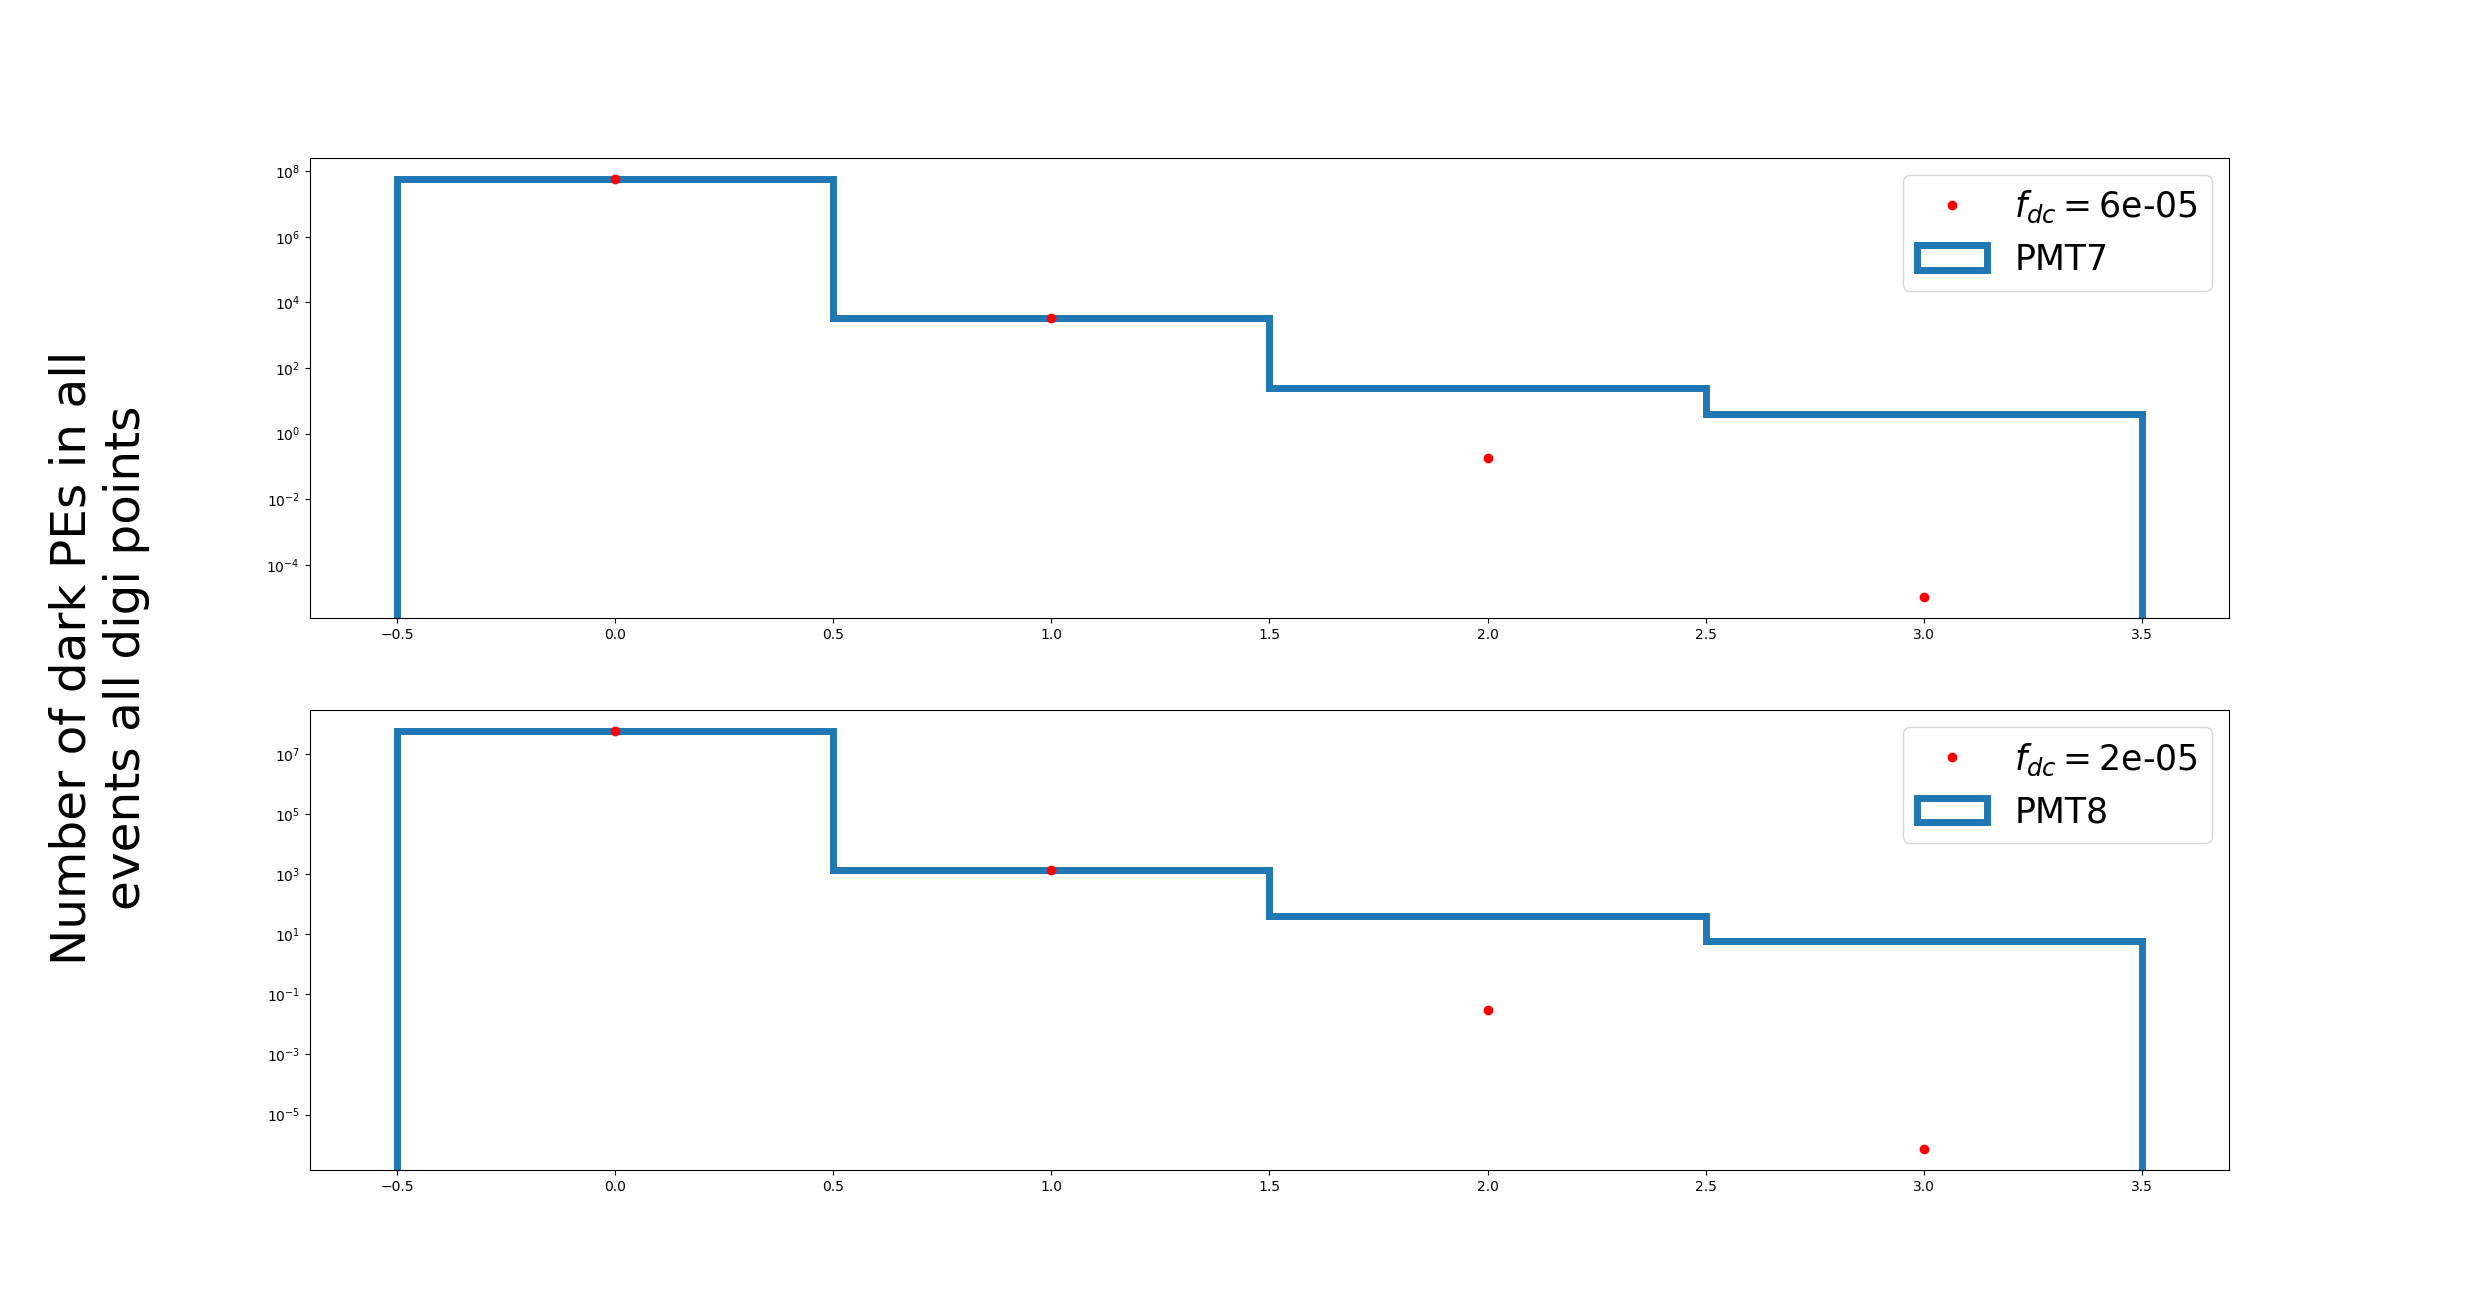
\includegraphics[width=0.75\textwidth]{f_dc.png}
\end{figure}
\end{frame}

\begin{frame}{Dark Current Correction to the Model}
\begin{equation}
\begin{split}
\tilde{H}_{0i}&\rightarrow \left(1-\frac{f_{dc}}{1-f_{dc}}\right)\tilde{H}_{0i}\\
\tilde{H}_{0i}&\rightarrow \left(1-\frac{f_{dc}}{1-f_{dc}}\right)\tilde{H}_{ni}+\sum_{m=1}^{n}f_{dc}^m\tilde{H}_{n-mi}
\end{split}
\end{equation}
This should be corrected before the alignment.
\end{frame}


\begin{frame}{Dark Current Correction to the Simulation}
For each digi point add a random number sampled with the probability
\begin{equation}
\begin{split}
&P(0)=1-\frac{1}{1-f_{dc}}\\
&P(n>0)=f_{dc}^n
\end{split}
\end{equation}
\end{frame}

\begin{frame}{Global Fit to Temporal structure, Delays Distribution and Dark Current Rate}
\begin{center}
\begin{figure}[h]
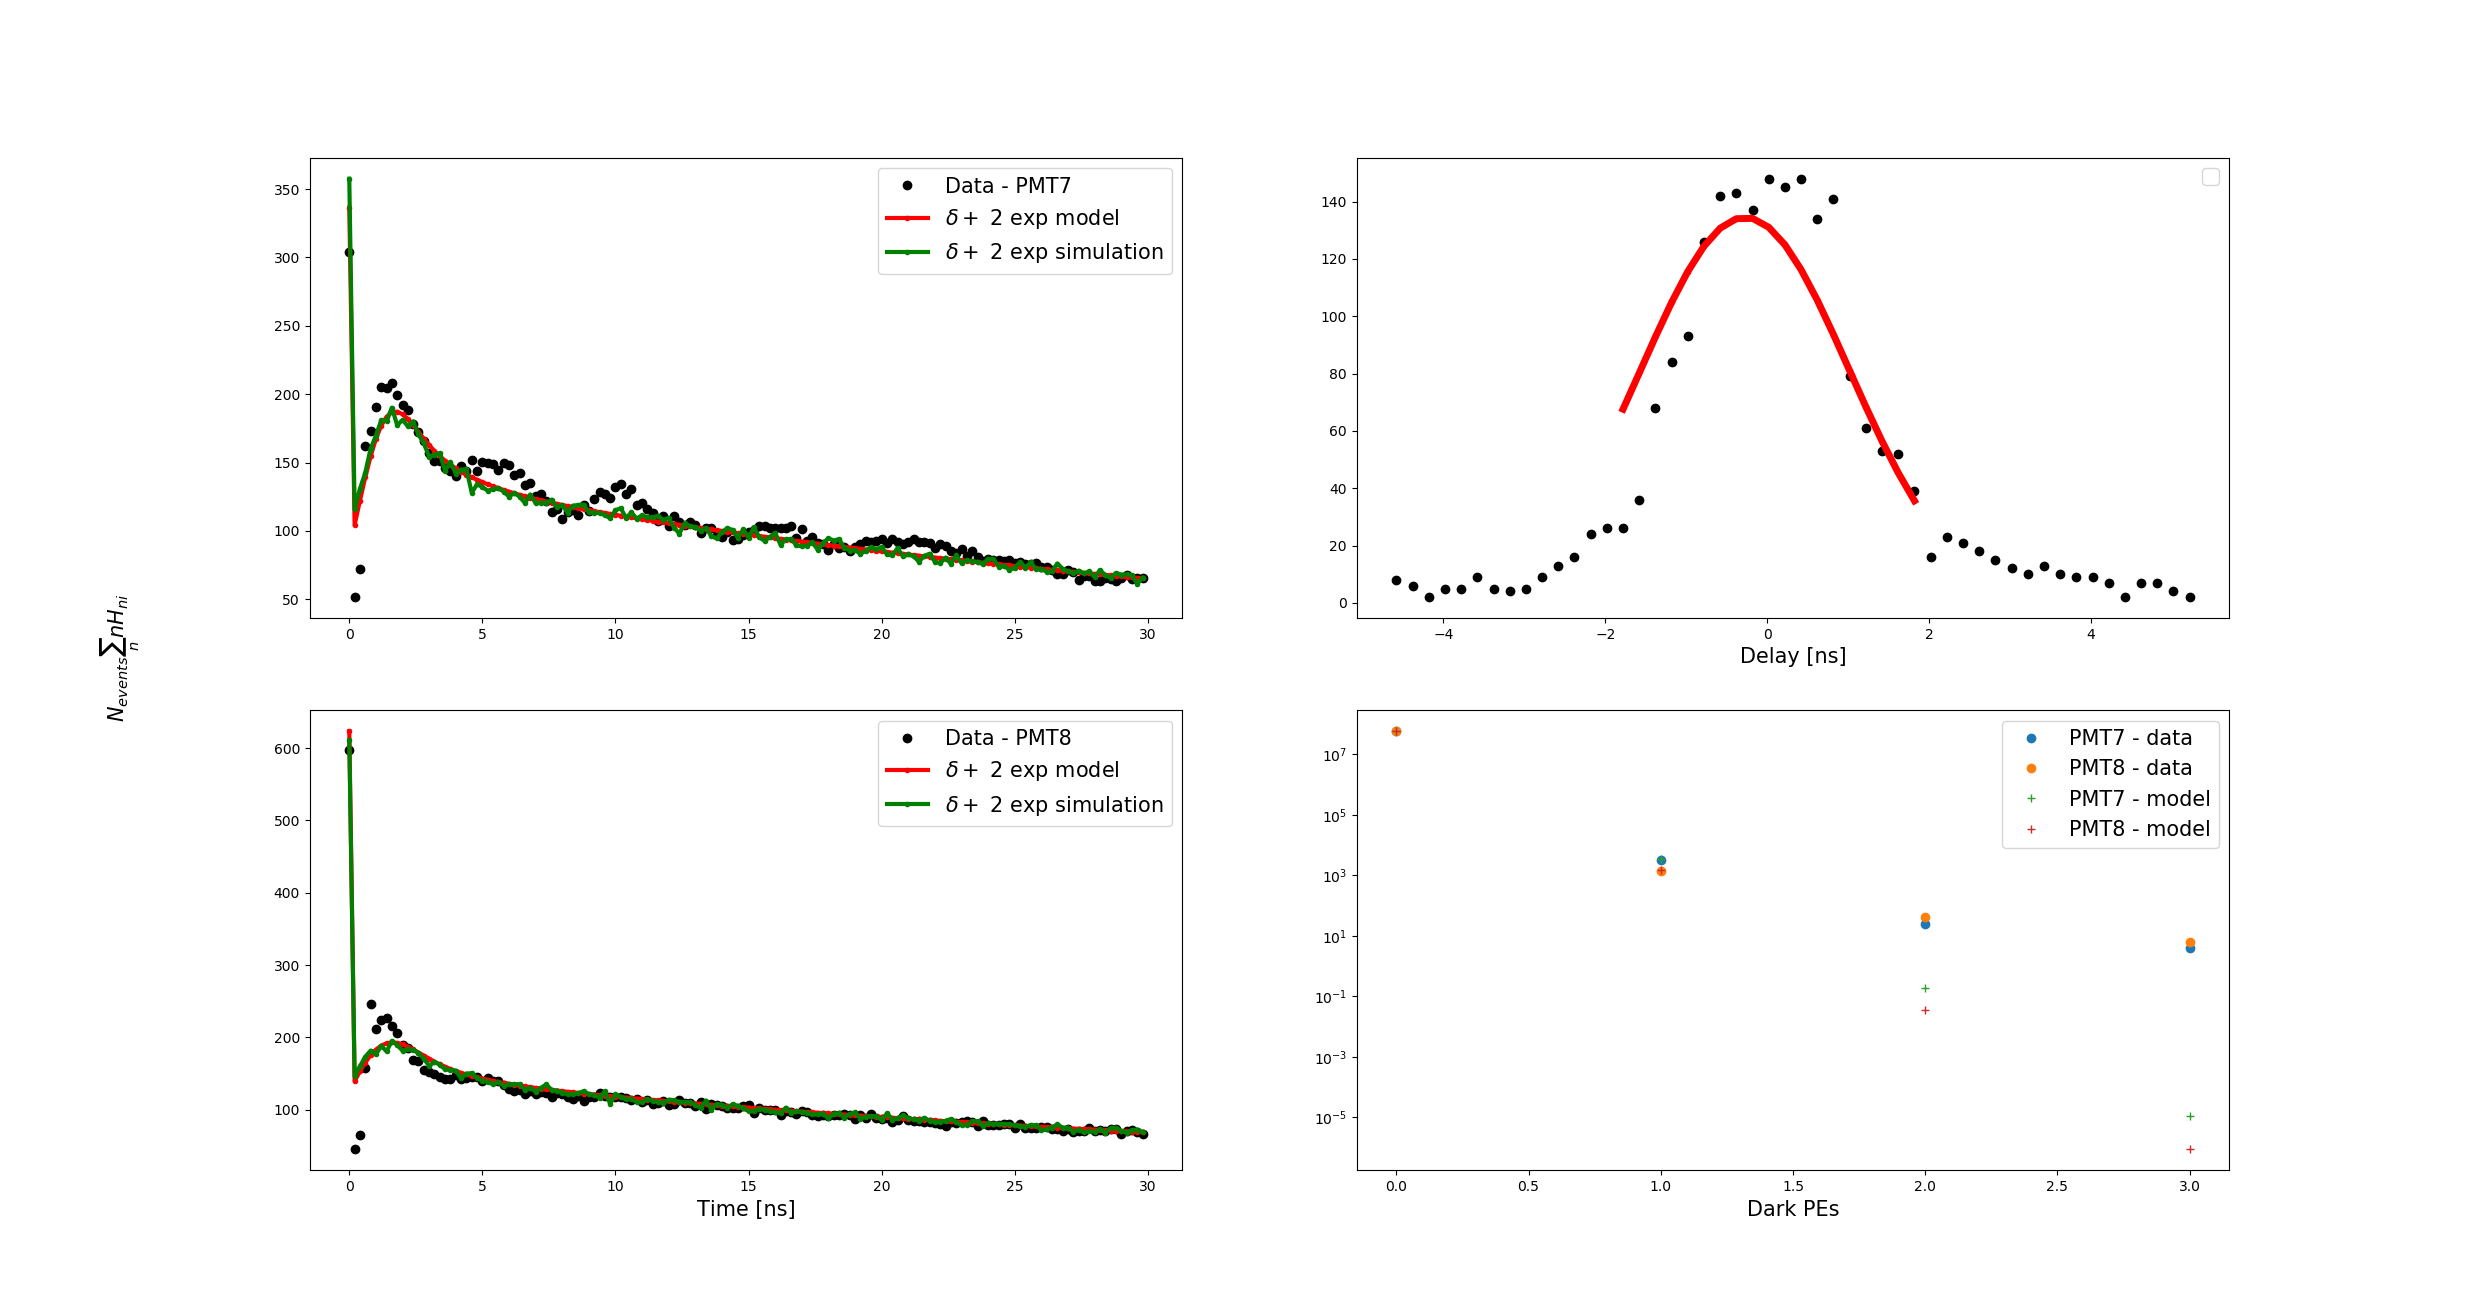
\includegraphics[width=1\textwidth]{fit4.png}
\end{figure}
\end{center}

\end{frame}

\begin{frame}{Global Fit to Temporal structure, Delays Distribution and Dark Current Rate}
\begin{center}
\begin{tabular}{|c||c|c|c|c|c|} 
\hline
PMT & $NQ$ & $T_0$ [ns]& $\sigma_t$ [ns] & $R$ & $f_{dc}$\\ 
\hline\hline
7 & 34 & 2 & 0.75 & 0.03  & $6\cdot10^{-5}$ \\
\hline
8 & 34 & 1.7 & 1 & 0.03 &  $2\cdot10^{-5}$ \\
\hline
\end{tabular}
\end{center}

\begin{center}
\begin{tabular}{|c|c|c|} 
\hline
$F$ & $\tau_f$ [ns]& $\tau_s$ [ns] \\ 
\hline\hline
0.02 & 1.76 & 37 \\
\hline
\end{tabular}
\end{center}

The $T_0$ parameter is weird but we don't really sensitive to it, only to the difference between the two values.
\end{frame}


\begin{frame}{Correction due the SPE resolution}
...
\end{frame}



\end{document}

